\def\sectiontitle{Benchmarks}

\section{\sectiontitle}

%%%%%%%%%%%%%%%%%%%%%%%%%%%%%%%%%%%%%%%%%%%%%%%%%%%%%%%%%%%%%%%%%%%%%%%%%%%%%%%%
\def\slidetitle{2-steps workflow}

\subsection{\slidetitle}
\begin{frame}
  \frametitle{\sectiontitle}
  \framesubtitle{\slidetitle}

  \begin{minipage}[h!]{0.35\textwidth}

    WIPP 2-steps workflow

    \begin{enumerate}
        \item Inference the model
        \item Compute the accuracy
    \end{enumerate}

  \end{minipage}\hfill
  \begin{minipage}[h!]{0.65\textwidth}
    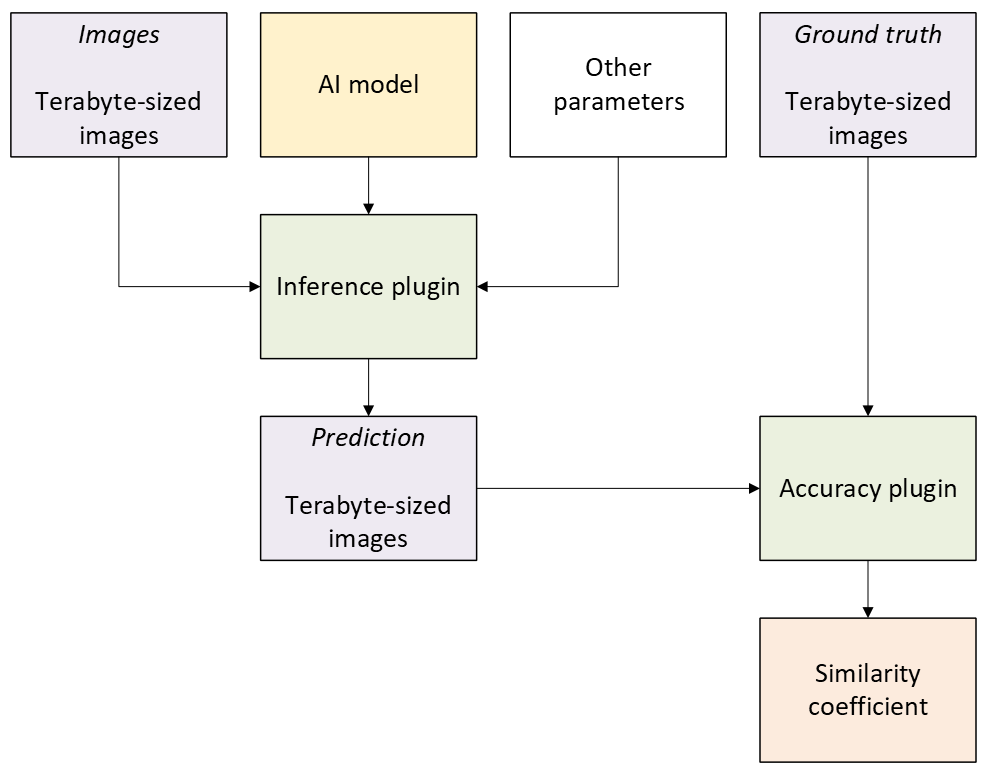
\includegraphics[scale=0.52]{./img/3_benchmark/workflow.png}
  \end{minipage}
\end{frame}

%%%%%%%%%%%%%%%%%%%%%%%%%%%%%%%%%%%%%%%%%%%%%%%%%%%%%%%%%%%%%%%%%%%%%%%%%%%%%%%%
\def\slidetitle{Data 'cell boundary'}

\subsection{\slidetitle}
\begin{frame}
  \frametitle{\sectiontitle}
  \framesubtitle{\slidetitle}

  \begin{minipage}[h!]{0.40\textwidth}
    Name: Retinal Pigment Epithelium

    Number: 1032 images (822/210)

    \centering
    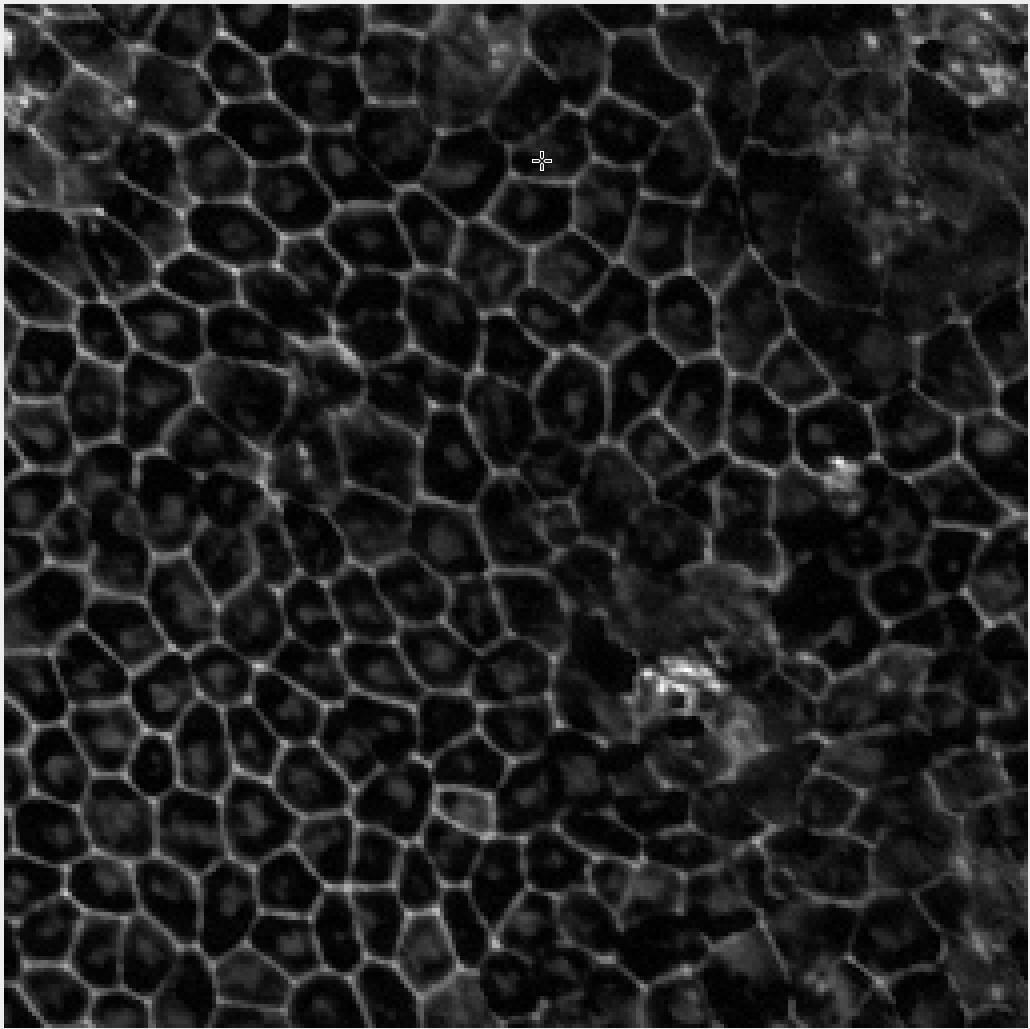
\includegraphics[scale=0.13]{./img/3_benchmark/image.png}
    \textbf{Image}
  \end{minipage}\hfill
  \begin{minipage}[h!]{0.40\textwidth}
    Type: Cell microscopy

    Size: 256x256

    \centering
    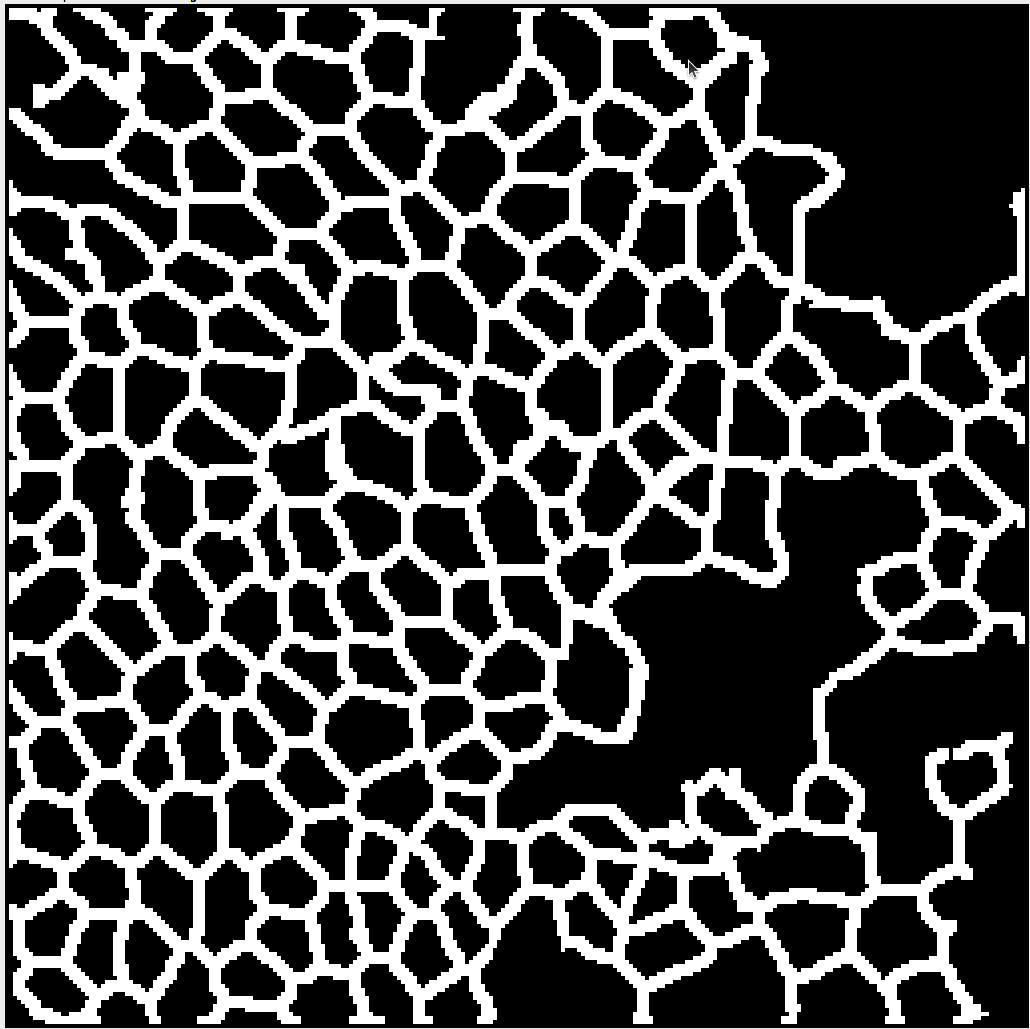
\includegraphics[scale=0.13]{./img/3_benchmark/mask.png}
    \textbf{Mask}
  \end{minipage}

  \bigskip

  Source: https://doi.org/doi:10.18434/T4/1503229

\end{frame}

%%%%%%%%%%%%%%%%%%%%%%%%%%%%%%%%%%%%%%%%%%%%%%%%%%%%%%%%%%%%%%%%%%%%%%%%%%%%%%%%
\def\slidetitle{Accuracy for 'cell boundary'}

\subsection{\slidetitle}
\begin{frame}
  \frametitle{\sectiontitle}
  \framesubtitle{\slidetitle}

  Compute time: Few minutes on WIPP

  Task: Segments cell edges

  \begin{center}
    \begin{table}
      \begin{tabular}{|l|l|c|}
       \hline
       \rowcolor{tableFirstRowColor}  Repository    & Model                       & Accuracy \\ [0.5ex]
       \hline
       \cellcolor{tableFirstColColor} WIPP          & unet-cnn*                   & 95.11\% $\pm$ 0.78\% \\
       \hline
       \cellcolor{tableFirstColColor} BioImage.IO   & 10.5281/zenodo.5869899      & 89.30\% $\pm$ 0.84\% \\
       \hline
       \cellcolor{tableFirstColColor} Hugging Face  & facebook/sam-vit-huge       & 86.01\% $\pm$ 2.50\% \\
       \hline
       \hline
       \cellcolor{tableFirstColColor} SAM2          & facebook/sam2.1-hiera-large & 80.18\% $\pm$ 5.02\% \\
       \hline
       \cellcolor{tableFirstColColor} Cellpose      & cyto3                       & 78.51\% $\pm$ 2.35\% \\
       \hline
      \end{tabular}
      \caption{Models accuracy after inference on data 'cell boundary'}
    \end{table}
  \end{center}

  *Trained with data, then inferenced (in WIPP)

\end{frame}

%%%%%%%%%%%%%%%%%%%%%%%%%%%%%%%%%%%%%%%%%%%%%%%%%%%%%%%%%%%%%%%%%%%%%%%%%%%%%%%%
\def\slidetitle{Data 'nuclei segmentation'}

\subsection{\slidetitle}
\begin{frame}
  \frametitle{\sectiontitle}
  \framesubtitle{\slidetitle}

  \begin{minipage}[h!]{0.40\textwidth}
    Name: Data Science Bowl 2018

    Number: 497 images (447/50)

    \centering
    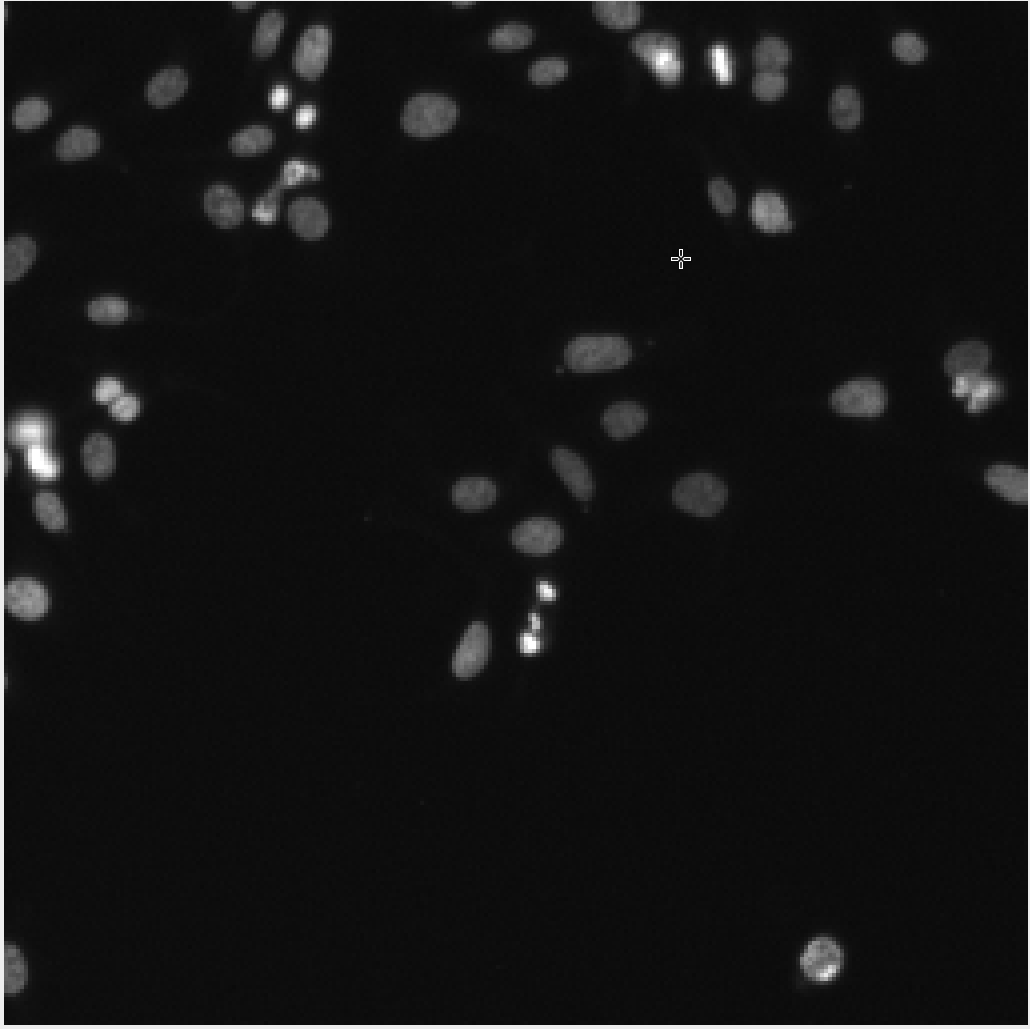
\includegraphics[scale=0.13]{./img/3_benchmark/image_2.png}
    \textbf{Image}
  \end{minipage}\hfill
  \begin{minipage}[h!]{0.40\textwidth}
    Type: Cell microscopy

    Size: 256x256 and 696x520

    \centering
    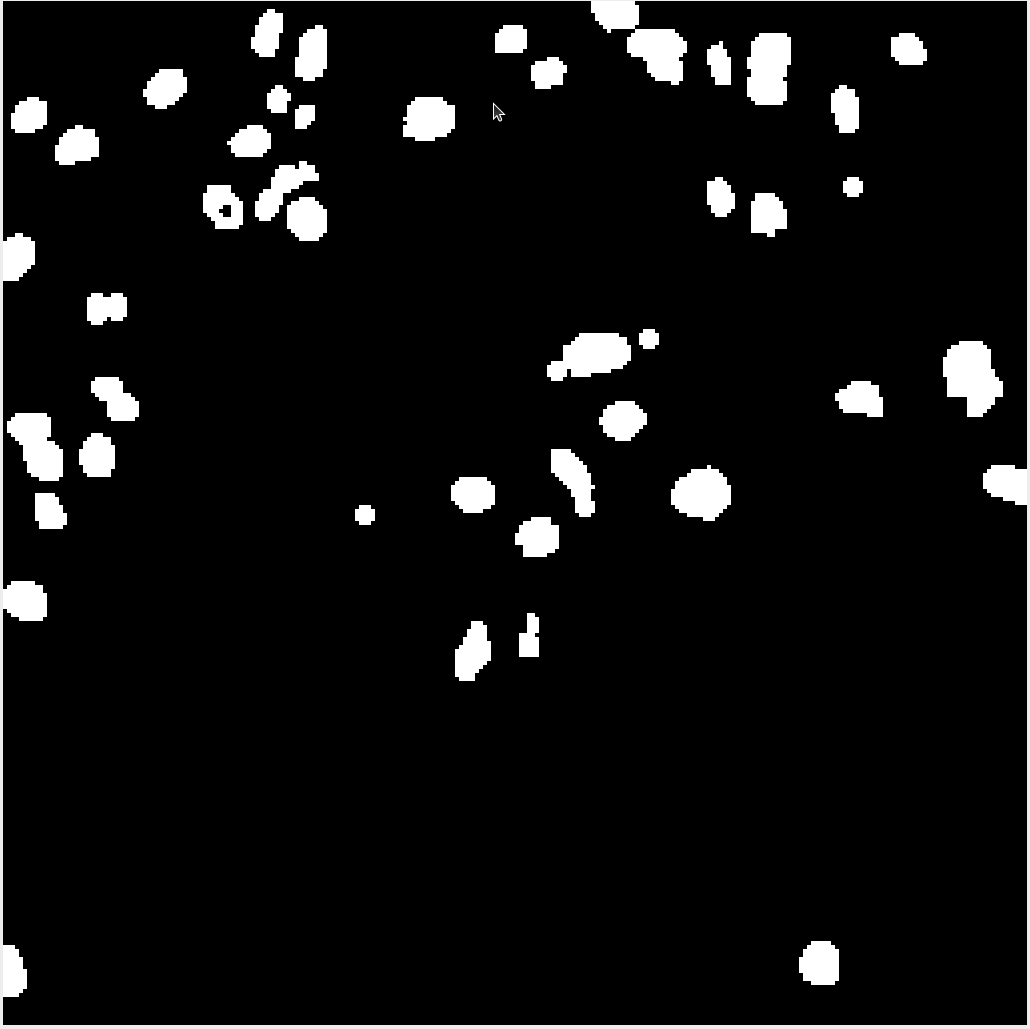
\includegraphics[scale=0.13]{./img/3_benchmark/mask_2.png}
    \textbf{Mask}
  \end{minipage}

  \bigskip

  Source: https://bbbc.broadinstitute.org/BBBC038/

\end{frame}

%%%%%%%%%%%%%%%%%%%%%%%%%%%%%%%%%%%%%%%%%%%%%%%%%%%%%%%%%%%%%%%%%%%%%%%%%%%%%%%%
\def\slidetitle{Accuracy for 'nuclei segmentation'}

\subsection{\slidetitle}
\begin{frame}
  \frametitle{\sectiontitle}
  \framesubtitle{\slidetitle}

  Compute time: Few minutes on WIPP

  Task: Segments nuclei of cells

  \begin{center}
    \begin{table}
        \begin{tabular}{|l|l|c|}
            \hline
            \rowcolor{tableFirstRowColor}  Repository   & Model                         & Accuracy \\ [0.5ex]
            \hline
            \cellcolor{tableFirstColColor} BioImage.IO  & 10.5281/zenodo.5764892        & 93.73\% $\pm$ 3.98\% \\
            \hline
            \cellcolor{tableFirstColColor} WIPP         & Stardist 2D paper DSB 2018    & 90.67\% $\pm$ 4.42\% \\
            \hline
            \cellcolor{tableFirstColColor} Cellpose     & cyto3                         & 82.31\% $\pm$ 17.25\% \\
            \hline
            \cellcolor{tableFirstColColor} Cellpose     & nuclei                        & 81.00\% $\pm$ 21.00\% \\
            \hline
            \hline
            \cellcolor{tableFirstColColor} SAM2         & facebook/sam2.1-hiera-small   & 48.18\% $\pm$ 32.41\% \\
            \hline
            %\cellcolor{tableFirstColColor} SAM2         & facebook/sam2.1-hiera-large   & 33.89\% $\pm$ 29.43\% \\
            %\hline
            \cellcolor{tableFirstColColor} BioImage.IO  & 10.5281/zenodo.5869899        & 29.47\% $\pm$ 8.32\% \\
            \hline
            \cellcolor{tableFirstColColor} Hugging Face & facebook/sam-vit-huge         & 21.63\% $\pm$ 15.37\% \\
            \hline
        \end{tabular}
      \caption{Models accuracy after inference on data 'nuclei segmentation'}
    \end{table}
  \end{center}

\end{frame}

\iffalse
%%%%%%%%%%%%%%%%%%%%%%%%%%%%%%%%%%%%%%%%%%%%%%%%%%%%%%%%%%%%%%%%%%%%%%%%%%%%%%%%
\def\slidetitle{Present 3D data}

\subsection{\slidetitle}
\begin{frame}
  \frametitle{\sectiontitle}
  \framesubtitle{\slidetitle}

  TODO

\end{frame}

%%%%%%%%%%%%%%%%%%%%%%%%%%%%%%%%%%%%%%%%%%%%%%%%%%%%%%%%%%%%%%%%%%%%%%%%%%%%%%%%
\def\slidetitle{Benchmark 3D data}

\subsection{\slidetitle}
\begin{frame}
  \frametitle{\sectiontitle}
  \framesubtitle{\slidetitle}

  Compute in few minutes on WIPP with dataset `3D-RPE W3`

  The first column (gray) is ground truth and the first row (blue) is model prediction

  \begin{center}
    \begin{table}
      \begin{tabular}{|c|c|c|c|c|}
       \hline
       \rowcolor{tableFirstRowColor}      & Wipp unet             & BioImage.IO*          & Cellpose cyto3        & Sam2**   \\ [0.5ex]
       \hline
       \cellcolor{tableFirstColColor} W3  & 83.97\% $\pm$ 14.95\% & 52.05\% $\pm$ 31.57\% & 49.53\% $\pm$ 25.06\% & 30.18\% $\pm$ 27.09\% \\
       \hline
       \cellcolor{tableFirstColColor} W   & $\times$              & 54.99\% $\pm$ 31.74\% & 51.75\% $\pm$ 25.33\% & 31.60\% $\pm$ 27.91\% \\
       \hline
       \cellcolor{tableFirstColColor} B   & $\times$              & $\times$              & 71.48\% $\pm$ 14.09\% & 51.76\% $\pm$ 22.86\% \\
       \hline
       \cellcolor{tableFirstColColor} C   & $\times$              & $\times$              & $\times$              & 51.29\% $\pm$ 27.54\% \\
       \hline
      \end{tabular}
      \caption{Similarity across different models and ground truth}
    \end{table}
  \end{center}

  *NucleiSegmentationBoundaryModel (10.5281/zenodo.5764892)

  **sam2-hiera-large

\end{frame}

%%%%%%%%%%%%%%%%%%%%%%%%%%%%%%%%%%%%%%%%%%%%%%%%%%%%%%%%%%%%%%%%%%%%%%%%%%%%%%%%
\def\slidetitle{Explaining poor 3D results}

\subsection{\slidetitle}
\begin{frame}
  \frametitle{\sectiontitle}
  \framesubtitle{\slidetitle}

  \begin{minipage}[h!]{0.30\textwidth}
    \centering
    \textbf{Image (example)}\par\medskip
    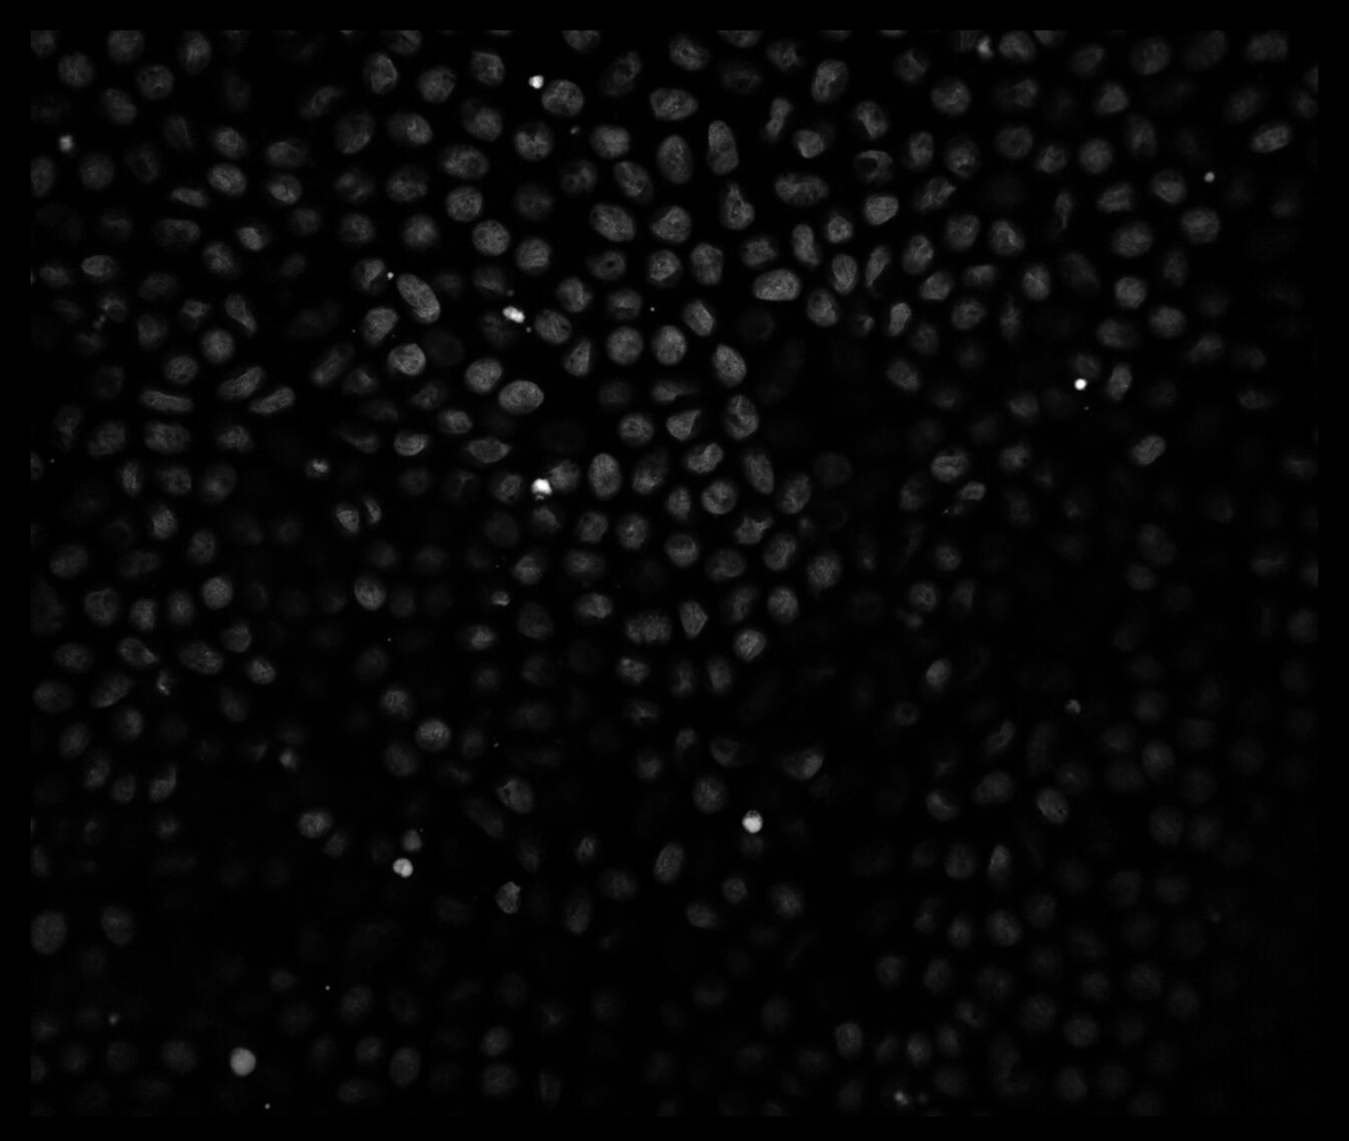
\includegraphics[scale=0.1]{./img/result_img.png}
  \end{minipage}\hfill
  \begin{minipage}[h!]{0.30\textwidth}
    \centering
    \textbf{Mask (associated)}\par\medskip
    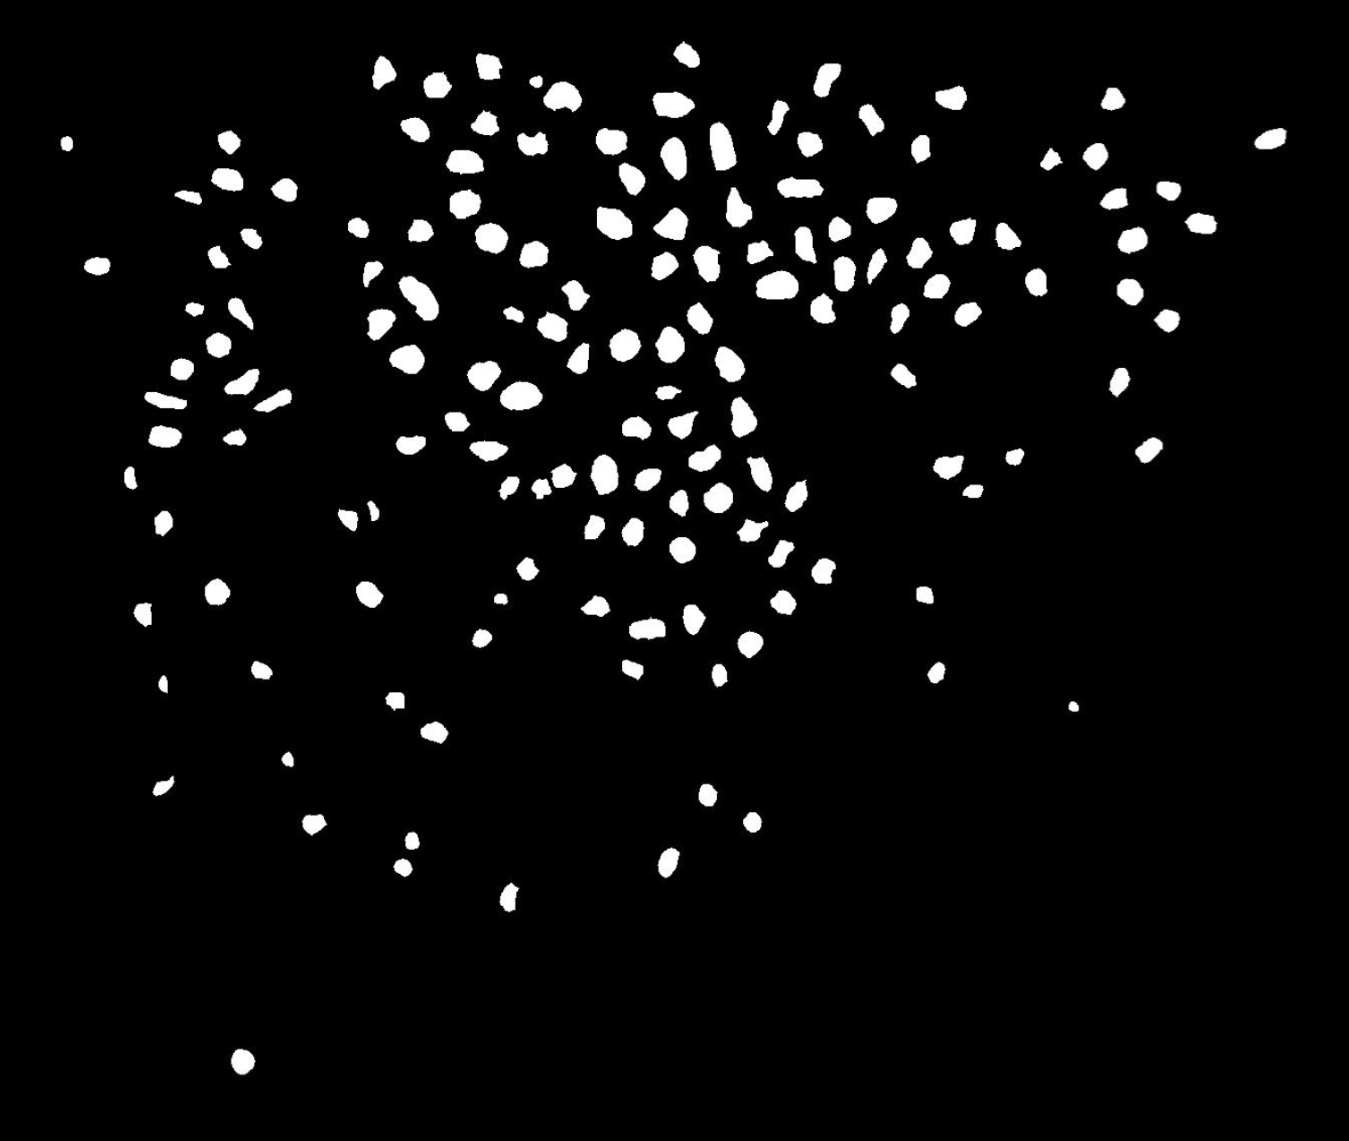
\includegraphics[scale=0.1]{./img/result_mask.png}
  \end{minipage}\hfill
  \begin{minipage}[h!]{0.30\textwidth}
    \centering
    \textbf{Prediction (B model)}\par\medskip
    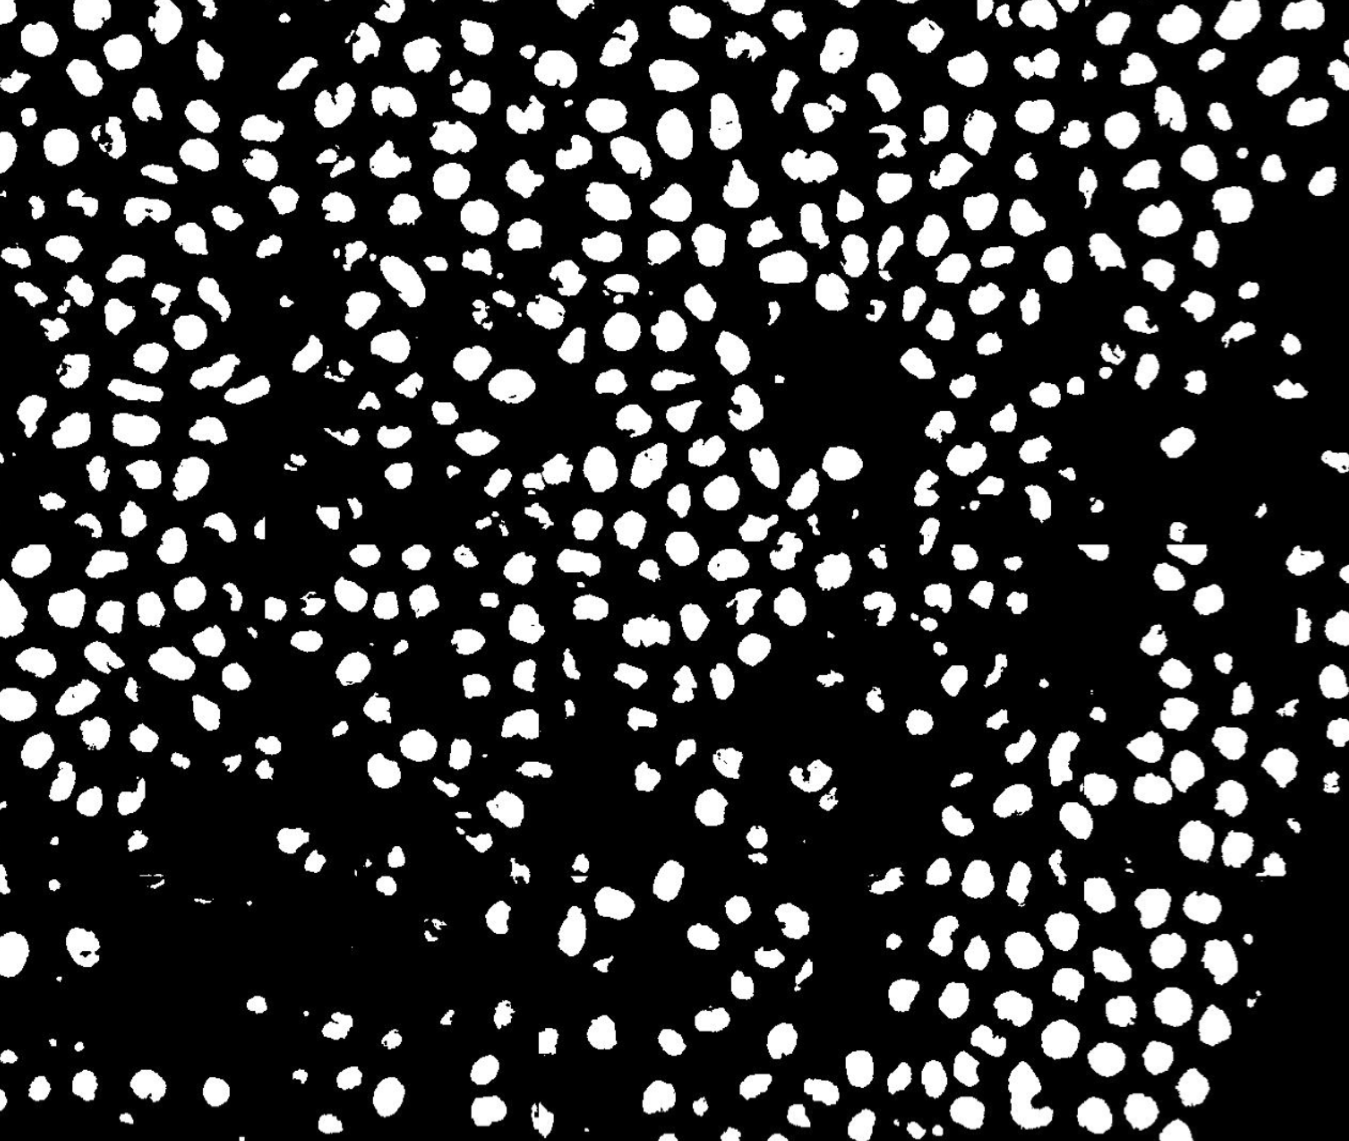
\includegraphics[scale=0.1]{./img/result_pred_bio.png}
  \end{minipage}

  \medskip
  Memo: With other, more conventional 2D data, the results are much better!

\end{frame}
\fi
